% Copyright (c) 2021-10-07 Eclipse Arrowhead Project
%
% This program and the accompanying materials are made available under the
% terms of the Eclipse Public License 2.0 which is available at
% http://www.eclipse.org/legal/epl-2.0.
%
% SPDX-License-Identifier: EPL-2.0

This section is what constitutes the \GlossaryHyperRef{model-reference}{reference model} of this document.
Each of its subsections \GlossaryHyperRef{description}{describes} a primary Arrowhead concept, which are as follows:

\vspace*{0.25cm}
\begin{itemize}[leftmargin=1.2cm,rightmargin=0pt,labelwidth=1cm,labelsep=0pt,itemindent=0pt,parsep=0pt,topsep=0pt,align=left]
\item[\ref{sec:reference-model:stakeholder}] \textbf{\nameref{sec:reference-model:stakeholder}}
\item[\ref{sec:reference-model:entity}] \textbf{\nameref{sec:reference-model:entity}}
\item[\ref{sec:reference-model:device}] \textbf{\nameref{sec:reference-model:device}}
\item[\ref{sec:reference-model:system}] \textbf{\nameref{sec:reference-model:system}}
\item[\ref{sec:reference-model:service}] \textbf{\nameref{sec:reference-model:service}}
\item[\ref{sec:reference-model:system-of-systems}] \textbf{\nameref{sec:reference-model:system-of-systems}}
\vspace*{0.1cm}
\begin{itemize}[leftmargin=1cm,rightmargin=0pt,labelwidth=1cm,labelsep=0pt,itemindent=0pt,parsep=0.05cm,topsep=0.05cm,align=left]
  \item[\ref{sec:reference-model:system-of-systems:local-cloud}] \textbf{\nameref{sec:reference-model:system-of-systems:local-cloud}}
  \item[\ref{sec:reference-model:system-of-systems:system-of-local-clouds}] \textbf{\nameref{sec:reference-model:system-of-systems:system-of-local-clouds}}
\end{itemize}
\vspace*{0.1cm}
\item[\ref{sec:reference-model:network}] \textbf{\nameref{sec:reference-model:network}}
\item[\ref{sec:reference-model:interface}] \textbf{\nameref{sec:reference-model:interface}}
\item[\ref{sec:reference-model:policy}] \textbf{\nameref{sec:reference-model:policy}}
\item[\ref{sec:reference-model:protocol}] \textbf{\nameref{sec:reference-model:protocol}}
\item[\ref{sec:reference-model:data}] \textbf{\nameref{sec:reference-model:data}}
\end{itemize}
\vspace*{0.25cm}

\subsection{Stakeholder}
\label{sec:reference-model:stakeholder}

A \GlossaryHyperRef{stakeholder}{stakeholder} is a person or \GlossaryHyperRef{organization}{organization} with \GlossaryHyperRef{stake}{stake} in an \GlossaryHyperRef{entity}{entity} or undertaking with relevance to the \GlossaryHyperRef{framework-arrowhead}{Arrowhead framework}.
In this context, we understand \textit{stake} to refer to any type of engagement or commitment.
The concept is illustrated in Figure \ref{fig:stakeholder}, which also lists five reasons why a given person or organization could be considered to be a stakeholder.
We refer to these reasons as \GlossaryHyperRef{role-stakeholder}{\textit{roles}}.

\begin{figure}[ht!]
  \centering
  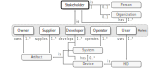
\includegraphics{figures/stakeholder}
  \caption{
    The stakeholder as either a person or organization, where each such stakeholder takes on one ore more distinct roles.
    The depicted roles is not an exhaustive list.
    \GlossaryHyperRef{hid}{HID} is an abbreviation for \GlossaryHyperRef{device-human-interface}{Human Interface Device}.
  }
  \label{fig:stakeholder}
\end{figure}

The roles occupied by a given stakeholder dictates what \GlossaryHyperRef{entity}{entities} that person or organization will interact with, as well as the nature of that interaction.
In Figure \ref{fig:stakeholder}, (1) \GlossaryHyperRef{owner}{owner}, (2) \GlossaryHyperRef{designer}{designer}, (3) \GlossaryHyperRef{developer}{developer}, (4) \GlossaryHyperRef{operator}{operator} and (5) \GlossaryHyperRef{user}{user} are named explicitly, but more roles are likely to be relevant.
Use of the listed five names is preferred over any synonyms when referring to these particular roles.
Refer to the \hyperref[sec:glossary]{glossary} for their definitions.

\subsection{Entity}
\label{sec:reference-model:entity}

An \GlossaryHyperRef{entity}{entity} is an \GlossaryHyperRef{artifact}{artifact} that can be distinguished from all other artifacts.
We use the word \textit{artifact} to refer to any object or thing, physical or intangible.
As depicted in Figure \ref{fig:entity}, this means that an entity always has an \GlossaryHyperRef{identity}{identity}.

\begin{figure}[ht!]
  \centering
  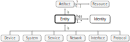
\includegraphics{figures/entity}
  \caption{
    The entity as an artifact with an identity.
    An entity or artifact may or may not be considered to be a \GlossaryHyperRef{resource}{resource}, in which case it is deemed to be of value to a \GlossaryHyperRef{stakeholder}{stakeholder}.
    The group of entity types is not exhaustive.
    Other examples are \GlossaryHyperRef{cloud-local}{local clouds}, certain \GlossaryHyperRef{data}{data}, \GlossaryHyperRef{policy}{policies}, \GlossaryHyperRef{protocol}{protocols} and \GlossaryHyperRef{profile}{profiles}.
  }
  \label{fig:entity}
\end{figure}

Having an identity is not the same as being associated with an \GlossaryHyperRef{identifier}{identifier}, which is data, of any conceivable \GlossaryHyperRef{type-data}{type}, naming the entity in question.
As long as some form of \GlossaryHyperRef{description}{description} can be produced that unambiguously refers to the artifact in question, it has an identity.
That being said, certain \GlossaryHyperRef{identification}{identification} requirements, perhaps related to security, performance or discoverability, may make it practically unfeasible not to use identifiers.

\subsection{Device}
\label{sec:reference-model:device}

A \GlossaryHyperRef{device}{device} is a physical \GlossaryHyperRef{entity}{entity} that is able to automatically exercise at least one \GlossaryHyperRef{capability}{capability}.
A capability is some form of automation routine that can be performed if triggered by the \GlossaryHyperRef{software}{software} of the device.
Examples of capabilities include moving robotic arms, reading from sensors, starting software procedures, hosting \GlossaryHyperRef{system}{systems} and sending \GlossaryHyperRef{message}{messages}. 
Every device consists of \GlossaryHyperRef{components-hardware}{hardware components}, which are what concretely facilitate its capabilities.
While there are not limits to what components can make up a device, they must always have (1) \GlossaryHyperRef{memory}{memory}, (2) \GlossaryHyperRef{computer}{compute} and (3) \GlossaryHyperRef{interface-device}{interfacing} components, as shown in Figure \ref{fig:device}.

\begin{figure}[ht!]
  \centering
  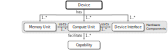
\includegraphics{figures/device}
  \caption{
    The device as an entity with hardware components, together facilitating one or more capabilities.
    The group of hardware components is not exhaustive.
    Other examples of such components could be sensors, actuators, compute accelerators, or batteries.
  }
  \label{fig:device}
\end{figure}

Devices may be able to host systems, in which case they may be referred to as \GlossaryHyperRef{device-system}{system devices}.
However, as it is rarely relevant to consider any other devices than those able to host systems, the ``system'' qualifier should be omitted if the context makes it clear that no other type of device is being referred to.
Devices that cannot host systems should be referred to with a leading qualifier that indicates why that is the case.
Examples of such qualifier could be ``constrained'', ``legacy'' or ``application-specific''.

\subsection{System}
\label{sec:reference-model:system}

A \GlossaryHyperRef{system}{system} is an \GlossaryHyperRef{entity}{entity} facilitated by \GlossaryHyperRef{software}{software} that is able to exercise the \GlossaryHyperRef{capability}{capabilities} of its hosting \GlossaryHyperRef{device}{device}.
As shown in Figure \ref{fig:system}, a system consists of at least three \GlossaryHyperRef{component-software}{software components}, which are (1) \GlossaryHyperRef{state-software}{state}, (2) \GlossaryHyperRef{procedure-software}{procedures} and (3) \GlossaryHyperRef{interface-system}{system interfaces}, out of which the last two are required.
These components correspond to and are facilitated by the (1) \GlossaryHyperRef{memory}{memory}, (2) \GlossaryHyperRef{computer}{compute} and (3) \GlossaryHyperRef{interface-device}{interfacing} components of the hosting device.

\begin{figure}[ht!]
  \centering
  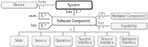
\includegraphics{figures/system}
  \caption{
    The system as a collection of related software components, able to trigger zero or more capabilities of its hosting device.
    The group of software components is not exhaustive.
    Other examples of such components could be operating systems, file systems, software libraries, programming language runtimes, databases or virtual machines.
  }
  \label{fig:system}
\end{figure}

Each system must have its own \GlossaryHyperRef{identity}{identity} and should be able to \GlossaryHyperRef{consumer-service}{consume} and/or \GlossaryHyperRef{provider-service}{provide} \GlossaryHyperRef{service}{services}.
There is no particular way in which a system must be facilitated.
They are not required to run in their own operating system processes, use any particular programming languages, virtual machines or databases, and so on.

\subsection{Service}
\label{sec:reference-model:service}

\begin{figure}[ht!]
  \centering
  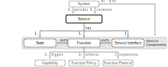
\includegraphics{figures/service}
  \caption{
    X
  }
  \label{fig:service}
\end{figure}

TODO: Explain function invocation. Separate diagram?

\subsection{System-of-Systems}
\label{sec:reference-model:system-of-systems}

\begin{figure}[ht!]
  \centering
  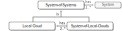
\includegraphics{figures/system-of-systems}
  \caption{
    X
  }
  \label{fig:system-of-systems}
\end{figure}

\subsubsection{Local Cloud}
\label{sec:reference-model:system-of-systems:local-cloud}

\begin{figure}[ht!]
  \centering
  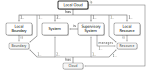
\includegraphics{figures/local-cloud}
  \caption{
    X
  }
  \label{fig:local-cloud}
\end{figure}

\subsubsection{System-of-Local-Clouds}
\label{sec:reference-model:system-of-systems:system-of-local-clouds}

X

\subsection{Network}
\label{sec:reference-model:network}

\begin{figure}[ht!]
  \centering
  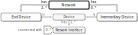
\includegraphics{figures/network}
  \caption{
    X
  }
  \label{fig:network}
\end{figure}

\subsection{Interface}
\label{sec:reference-model:interface}

\begin{figure}[ht!]
  \centering
  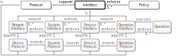
\includegraphics{figures/interface}
  \caption{
    X
  }
  \label{fig:interface}
\end{figure}

TODO: Discussion about difference between interface and service?

\subsection{Policy}
\label{sec:reference-model:policy}

\begin{figure}[ht!]
  \centering
  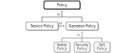
\includegraphics{figures/policy}
  \caption{
    X
  }
  \label{fig:policy}
\end{figure}

\subsection{Protocol}
\label{sec:reference-model:protocol}

\begin{figure}[ht!]
  \centering
  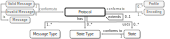
\includegraphics{figures/protocol}
  \caption{
    X
  }
  \label{fig:protocol}
\end{figure}


\subsection{Data}
\label{sec:reference-model:data}

\begin{figure}[ht!]
  \centering
  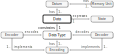
\includegraphics{figures/data}
  \caption{
    X
  }
  \label{fig:data}
\end{figure}